\documentclass[12pt,a4paper]{article}
\usepackage[utf8]{inputenc}
\usepackage[T1]{fontenc}
\usepackage{babel}
\usepackage{amsmath}
\usepackage{amsfonts}
\usepackage{amssymb}
\usepackage{graphicx}
\usepackage{hyperref}
\usepackage{booktabs}
\usepackage{listings}
\usepackage{color}

\definecolor{codegreen}{rgb}{0,0.6,0}
\definecolor{codegray}{rgb}{0.5,0.5,0.5}
\definecolor{codepurple}{rgb}{0.58,0,0.82}
\definecolor{backcolour}{rgb}{0.95,0.95,0.92}

\lstdefinestyle{mystyle}{
    backgroundcolor=\color{backcolour},   
    commentstyle=\color{codegreen},
    keywordstyle=\color{magenta},
    numberstyle=\tiny\color{codegray},
    stringstyle=\color{codepurple},
    basicstyle=\ttfamily\footnotesize,
    breakatwhitespace=false,         
    breaklines=true,                 
    captionpos=b,                    
    keepspaces=true,                 
    numbers=left,                    
    numbersep=5pt,                  
    showspaces=false,                
    showstringspaces=false,
    showtabs=false,                  
    tabsize=2
}
\lstset{style=mystyle}

\title{Trabajo 4 de Bases de Datos 2}
\author{}
\date{}

\begin{document}

\maketitle

\section{Introducción}
El objetivo de este trabajo es resolver y comparar varias formas de una misma consulta SQL: obtener todas las parejas de proveedores que venden exactamente el mismo conjunto de productos. La solución se desarrolla en Oracle y PostgreSQL, usando las mismas tablas y muestras de datos comparables.

El trabajo se hizo con Docker para que las pruebas puedan repetirse sin instalar manualmente los motores de base de datos en el sistema operativo.

\section{Objetivos}
\begin{itemize}
    \item Crear las tablas \texttt{Prov} y \texttt{ProvxProd} respetando la estructura del enunciado.
    \item Escribir cuatro consultas SQL distintas para resolver el problema.
    \item Crear un programa PL/SQL en Oracle que cargue datos aleatorios consistentes.
    \item Ejecutar pruebas con tamaños de muestra crecientes.
    \item Obtener Explain Plan y TKPROF en Oracle.
    \item Obtener métricas equivalentes en PostgreSQL mediante \texttt{EXPLAIN ANALYZE}.
    \item Comparar el comportamiento de las consultas en ambos motores.
\end{itemize}

\section{Modelo De Datos}
La tabla \texttt{Prov} almacena proveedores:
\begin{lstlisting}[language=SQL]
Prov(nit, nombre)
\end{lstlisting}

La tabla \texttt{ProvxProd} almacena los productos que vende cada proveedor:
\begin{lstlisting}[language=SQL]
ProvxProd(nit, codigoProducto)
\end{lstlisting}

Restricciones:
\begin{itemize}
    \item \texttt{Prov.nit} es clave primaria.
    \item \texttt{Prov.nombre} es único.
    \item \texttt{(ProvxProd.nit, ProvxProd.codigoProducto)} es clave primaria compuesta.
    \item \texttt{ProvxProd.nit} es clave foránea hacia \texttt{Prov}.
\end{itemize}
No se agregaron columnas adicionales porque el enunciado indica que no debe modificarse la estructura.

\section{Metodología}
Las pruebas se ejecutan con Docker Compose. Se levantan dos contenedores: Oracle Free y PostgreSQL.

Para cada muestra se realiza este proceso:
\begin{enumerate}
    \item Se eliminan los datos anteriores.
    \item Se cargan proveedores.
    \item Se cargan relaciones proveedor-producto aleatorias, evitando duplicados.
    \item Se ejecutan las cuatro consultas.
    \item En Oracle se genera Explain Plan.
    \item En Oracle se activa traza SQL y se procesa con TKPROF.
    \item En PostgreSQL se ejecuta \texttt{EXPLAIN (ANALYZE, BUFFERS)}.
    \item Se guardan los resultados en archivos de texto.
\end{enumerate}

Los tamaños de muestra propuestos son:
\begin{table}[h]
\centering
\begin{tabular}{|c|r|r|r|}
\hline
\textbf{Muestra} & \textbf{Proveedores} & \textbf{Productos posibles} & \textbf{Filas en ProvxProd} \\ \hline
1 & 100 & 1.000 & 1.000 \\ \hline
2 & 500 & 5.000 & 5.000 \\ \hline
3 & 1.000 & 10.000 & 10.000 \\ \hline
4 & 2.000 & 20.000 & 25.000 \\ \hline
5 & 5.000 & 50.000 & 50.000 \\ \hline
\end{tabular}
\end{table}

\section{Generación De Datos}
En Oracle se usa el procedimiento \texttt{cargar\_datos\_aleatorios}, escrito en PL/SQL. Primero borra los datos anteriores, luego inserta proveedores con \texttt{nit} consecutivo y nombre único. Después genera pares aleatorios \texttt{(nit, codigoProducto)}. Si un par ya existe, se ignora y se intenta generar otro.

La clave foránea siempre es consistente porque los valores de \texttt{nit} se generan entre 1 y el número de proveedores creados. También pueden quedar proveedores sin productos. Esto es correcto, porque el enunciado contempla el caso de proveedores con conjunto vacío de productos. (Los primeros 20 proveedores se dejan sin productos para garantizar los casos de conjunto vacío).

En PostgreSQL se implementa una versión equivalente en PL/pgSQL.

\section{Explicación De Las Cuatro Consultas}
\subsection{Consulta 1: doble NOT EXISTS}
Esta consulta compara cada pareja de proveedores \texttt{(p1, p2)}. La condición exige dos cosas: que no exista un producto vendido por \texttt{p1} que no venda \texttt{p2}, y viceversa. Esta consulta es distinta porque usa subconsultas correlacionadas y expresa la igualdad como ausencia de diferencias (división relacional).

\subsection{Consulta 2: agrupación y firma del conjunto}
Esta consulta crea una representación textual del conjunto de productos de cada proveedor (firma). En Oracle usa \texttt{LISTAGG}; en PostgreSQL usa \texttt{STRING\_AGG}. Los productos se ordenan antes de concatenarlos.

\textbf{Nota Técnica Importante:} En Oracle, el operador \texttt{LISTAGG} tiene un límite de 4000 bytes (o 32767 con tipos extendidos). Si un proveedor vendiera una cantidad masiva de productos, esto generaría el error \texttt{ORA-01489: result of string concatenation is too long}. Para este experimento, el número de productos por proveedor no excede el límite, pero en producción esto representa un riesgo de escalabilidad frente a enfoques puramente relacionales (como Q1 o Q3).

\subsection{Consulta 3: conteos y productos comunes}
Esta consulta calcula cuántos productos vende cada proveedor y cuántos tienen en común. Si tienen la misma cantidad total y los comunes coinciden con el total, venden el mismo conjunto. Es distinta porque se basa en agregaciones numéricas y no en operadores de conjuntos.

\subsection{Consulta 4: operadores de conjuntos}
En Oracle se usa \texttt{MINUS}; en PostgreSQL se usa \texttt{EXCEPT}. Revisa que las diferencias de conjuntos entre ambos proveedores sean vacías bidireccionalmente.

\section{Resultados y Análisis}
Todas las consultas retornaron 190 filas en todas las muestras, ya que se forzaron 20 proveedores sin productos, resultando en $20 \times 19 / 2 = 190$ parejas que comparten el conjunto vacío.

\subsection{Tablas de Resultados}

\subsubsection{Tabla Resumen Oracle - Explain Plan}
\begin{table}[h]
\centering
\resizebox{\textwidth}{!}{%
\begin{tabular}{|c|r|r|r|l|}
\hline
\textbf{Muestra} & \textbf{Consulta} & \textbf{Cost} & \textbf{Elapsed} & \textbf{Observaciones} \\ \hline
100 / 1.000 & Q1 - NOT EXISTS & 4472 & 0.01s & MERGE JOIN + FILTER, INDEX RANGE SCAN en PK\_PROVXPROD \\ \hline
100 / 1.000 & Q2 - LISTAGG & 218 & 0.00s & TEMP TABLE TRANSFORMATION, HASH JOIN a tabla temporal \\ \hline
100 / 1.000 & Q3 - conteos & 26 & 0.03s & TEMP TABLE TRANSFORMATION, HASH GROUP BY, NESTED LOOPS \\ \hline
100 / 1.000 & Q4 - MINUS & 3356 & 0.02s & MERGE JOIN + MINUS con INDEX RANGE SCAN \\ \hline
500 / 5.000 & Q1 - NOT EXISTS & 4472 & 0.21s & Mismo plan, costo no refleja el crecimiento de datos \\ \hline
500 / 5.000 & Q2 - LISTAGG & 220 & 0.00s & Plan estable, costo sube ligeramente \\ \hline
500 / 5.000 & Q3 - conteos & 30 & 0.71s & Mismo plan, NESTED LOOPS sobre 124.750 pares \\ \hline
500 / 5.000 & Q4 - MINUS & 3356 & 0.39s & Mismo plan, MINUS se ejecuta por cada par \\ \hline
1.000 / 10.000 & Q1 - NOT EXISTS & 4472 & 0.85s & Plan idéntico, tiempo real crece \\ \hline
1.000 / 10.000 & Q2 - LISTAGG & 224 & 0.00s & Plan estable y eficiente \\ \hline
1.000 / 10.000 & Q3 - conteos & 41 & 2.94s & Plan hash cambia a 2544319945 (full scan en Prov) \\ \hline
1.000 / 10.000 & Q4 - MINUS & 3356 & 1.58s & Mismo plan, 499.500 pares evaluados \\ \hline
2.000 / 25.000 & Q1 - NOT EXISTS & 4476 & 3.44s & Costo estimado apenas 4476, pero real 3.44s \\ \hline
2.000 / 25.000 & Q2 - LISTAGG & 234 & 0.02s & Plan estable, más rápido que Q1/Q3/Q4 por órdenes de magnitud \\ \hline
2.000 / 25.000 & Q3 - conteos & 63 & 16.40s & Usa disco (7335 lecturas físicas); alto costo real \\ \hline
2.000 / 25.000 & Q4 - MINUS & 3360 & 6.37s & 1.999.000 pares, 4.78M de LIOs \\ \hline
\end{tabular}%
}
\end{table}

\subsubsection{Tabla Resumen Oracle - Métricas (v\$sql)}
\begin{table}[h]
\centering
\resizebox{\textwidth}{!}{%
\begin{tabular}{|c|r|r|r|r|}
\hline
\textbf{Muestra} & \textbf{Consulta} & \textbf{LIOs / filas proc.} & \textbf{Filas ret. / fetches} & \textbf{Disco / LIOs} \\ \hline
100 / 1.000 & Q1 & 68.34 & 13.57 & 0.0000 \\ \hline
100 / 1.000 & Q2 & 0.09 & 13.57 & 0.0000 \\ \hline
100 / 1.000 & Q3 & 77.36 & 13.57 & 0.0000 \\ \hline
100 / 1.000 & Q4 & 69.43 & 13.57 & 0.0000 \\ \hline
500 / 5.000 & Q1 & 1,560.77 & 13.57 & 0.0000 \\ \hline
500 / 5.000 & Q2 & 0.12 & 13.57 & 0.0000 \\ \hline
500 / 5.000 & Q3 & 1,894.99 & 13.57 & 0.0000 \\ \hline
500 / 5.000 & Q4 & 1,563.44 & 13.57 & 0.0000 \\ \hline
1.000 / 10.000 & Q1 & 6,197.84 & 13.57 & 0.0000 \\ \hline
1.000 / 10.000 & Q2 & 0.20 & 13.57 & 0.0000 \\ \hline
1.000 / 10.000 & Q3 & 7,903.71 & 13.57 & 0.0000 \\ \hline
1.000 / 10.000 & Q4 & 6,201.65 & 13.57 & 0.0000 \\ \hline
2.000 / 25.000 & Q1 & 25,164.63 & 13.57 & 0.0000 \\ \hline
2.000 / 25.000 & Q2 & 0.41 & 13.57 & 0.0000 \\ \hline
2.000 / 25.000 & Q3 & 14,038.62 & 13.57 & 0.0027 \\ \hline
2.000 / 25.000 & Q4 & 25,193.05 & 13.57 & 0.0000 \\ \hline
\end{tabular}%
}
\end{table}

\subsubsection{Tabla Resumen PostgreSQL}
\begin{table}[h]
\centering
\resizebox{\textwidth}{!}{%
\begin{tabular}{|c|r|r|r|r|l|}
\hline
\textbf{Muestra} & \textbf{Consulta} & \textbf{Execution Time} & \textbf{shared hit} & \textbf{shared read} & \textbf{Observaciones} \\ \hline
100 / 1.000 & Q1 & 23.293 ms & 220 & 0 & Hash Anti Join, Nested Loop, Seq Scan + Index Scan \\ \hline
100 / 1.000 & Q2 & 0.721 ms & 9 & 0 & Hash Join con CTE, GroupAggregate \\ \hline
100 / 1.000 & Q3 & 10.954 ms & 216 & 0 & Hash Join con CTE, HashAggregate, Nested Loop \\ \hline
100 / 1.000 & Q4 & 74.343 ms & 69.881 & 0 & Nested Loop, SubPlan con HashSetOp Except \\ \hline
500 / 5.000 & Q1 & 60.035 ms & 2.522 & 0 & Mismo plan; 500 x 250 filas en Nested Loop \\ \hline
500 / 5.000 & Q2 & 3.079 ms & 34 & 0 & Plan eficiente, firma por STRING\_AGG \\ \hline
500 / 5.000 & Q3 & 207.707 ms & 2.499 & 0 & Hash Right Join produce 1.2M filas intermedias \\ \hline
500 / 5.000 & Q4 & 1.762.754 ms & 2.824.693 & 0 & SubPlan se ejecuta 124.750 veces; 2.8M buffers \\ \hline
1.000 / 10.000 & Q1 & 208.851 ms & 200.728 & 0 & Nested Loop produce 499.500 filas internas \\ \hline
1.000 / 10.000 & Q2 & 6.774 ms & 85 & 0 & Plan estable, 10.020 filas agrupadas \\ \hline
1.000 / 10.000 & Q3 & 951.194 ms & 199.433 & temp: 1511 & Usa disco por primera vez (hash batches: 4) \\ \hline
1.000 / 10.000 & Q4 & 7.946.117 ms & 15.862.912 & 0 & 499.500 iteraciones del SubPlan; 15.8M buffers \\ \hline
2.000 / 25.000 & Q1 & 801.607 ms & 398.426 & 0 & 1.999.000 filas en Nested Loop; JIT habilitado \\ \hline
2.000 / 25.000 & Q2 & 17.639 ms & 183 & 0 & Plan cambia a Merge Join (antes Hash Join) \\ \hline
2.000 / 25.000 & Q3 & 4.030.356 ms & 396.940 & temp: 10128 & 32 batches hash, 24.6M filas intermedias \\ \hline
2.000 / 25.000 & Q4 & 19.167.849 ms & 34.839.945 & 0 & 1.999.000 iteraciones, Index Only Scan, 34.8M buffers \\ \hline
\end{tabular}%
}
\end{table}

\subsection{Comparación de Rendimiento (Oracle vs PostgreSQL)}
\subsubsection{Tiempo de ejecución}
La consulta más rápida fue Q2 (\texttt{LISTAGG} / \texttt{STRING\_AGG}). Se mantuvo muy rápida (menor a 20 ms en Postgres y menor a 0.02s en Oracle) a pesar del crecimiento de la muestra.
La consulta más lenta fue Q4 (\texttt{MINUS} / \texttt{EXCEPT}), llegando a 19.17s en PostgreSQL con 2.000 proveedores.

\subsubsection{Lecturas lógicas y Planes de Ejecución}
La enorme diferencia de rendimiento en Q4 (donde PostgreSQL procesó 34.8M de \textit{shared hits} vs Oracle con 4.78M \textit{LIOs}) radica en el plan de ejecución:
\begin{itemize}
    \item \textbf{PostgreSQL} anida el \texttt{EXCEPT} en un \textit{SubPlan} evaluado exhaustivamente por cada pareja.
    \item \textbf{Oracle} utiliza un \texttt{INDEX RANGE SCAN} dentro de la operación \texttt{MINUS}. Esto ocurre porque Oracle aprovecha el índice compuesto (B-Tree) generado automáticamente en la Llave Primaria \texttt{ProvxProd(nit, codigoProducto)}. Al ser \texttt{nit} el primer atributo del índice, la base de datos puede resolver el \texttt{MINUS} mediante un \textit{Index Only Scan}, sin necesidad de acceder a los bloques de la tabla.
\end{itemize}

\section{Conclusiones}
\begin{enumerate}
    \item \textbf{La consulta más eficiente} fue Q2 (Firma con agregación de strings). Transformar un problema de conjuntos relacionales a un problema escalar evita el crecimiento cuadrático. Sin embargo, tiene la limitación de la longitud de bytes en Oracle.
    \item \textbf{Operadores de conjuntos (MINUS / EXCEPT)}: Fueron los enfoques más intuitivos, pero los de peor rendimiento.
    \item \textbf{El crecimiento cuadrático}: El problema base implica comparar combinaciones de $N$ elementos ($N \times (N-1) / 2$). Q1, Q3 y Q4 escalan muy mal con grandes volúmenes.
    \item \textbf{Oracle vs PostgreSQL}: Oracle supo aprovechar sus índices por defecto de manera más eficiente en los operadores \texttt{MINUS}, mientras que PostgreSQL fue superior en la manipulación rápida de \texttt{STRING\_AGG}.
\end{enumerate}

\section{Evidencias en PostgreSQL (Pantallazos)}
A continuación se presentan los pantallazos solicitados en el enunciado que evidencian la ejecución de las pruebas y la obtención de métricas en PostgreSQL de forma local:

\begin{figure}[htbp]
    \centering
    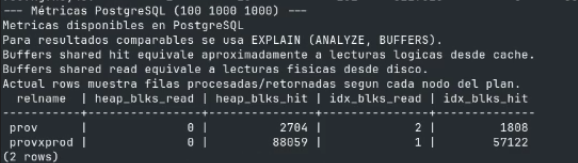
\includegraphics[width=0.8\textwidth]{../img/metricas_100.png}
    \caption{Métricas PostgreSQL - Muestra 100 proveedores}
\end{figure}

\begin{figure}[htbp]
    \centering
    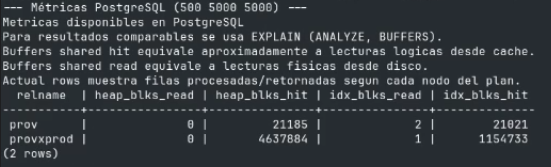
\includegraphics[width=0.8\textwidth]{../img/metricas_500.png}
    \caption{Métricas PostgreSQL - Muestra 500 proveedores}
\end{figure}

\begin{figure}[htbp]
    \centering
    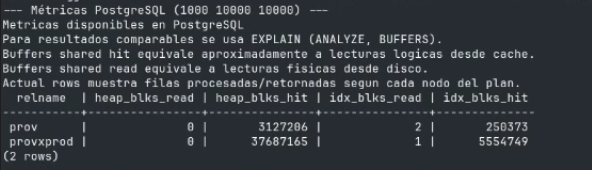
\includegraphics[width=0.8\textwidth]{../img/metricas_1000.png}
    \caption{Métricas PostgreSQL - Muestra 1000 proveedores}
\end{figure}

\begin{figure}[htbp]
    \centering
    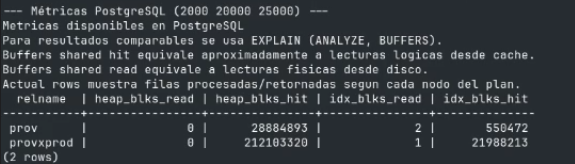
\includegraphics[width=0.8\textwidth]{../img/metricas_2000.png}
    \caption{Métricas PostgreSQL - Muestra 2000 proveedores}
\end{figure}

\begin{figure}[htbp]
    \centering
    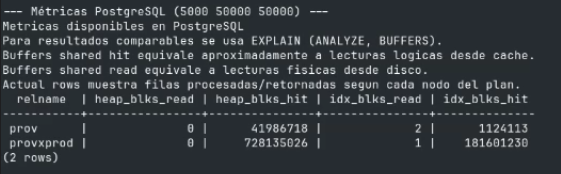
\includegraphics[width=0.8\textwidth]{../img/metricas_5000.png}
    \caption{Métricas PostgreSQL - Muestra 5000 proveedores}
\end{figure}

\begin{figure}[htbp]
    \centering
    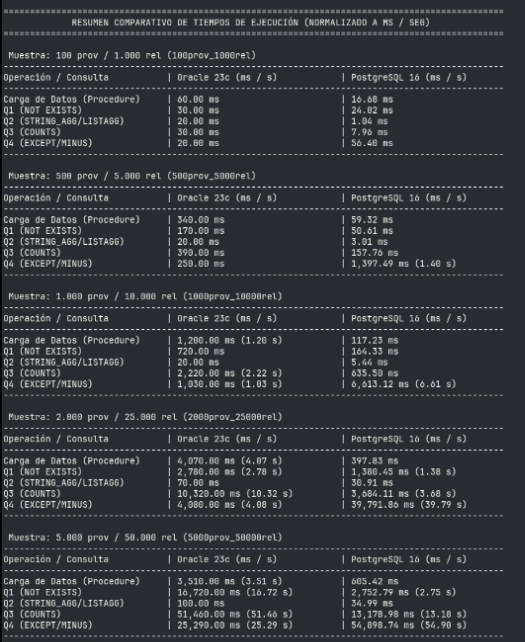
\includegraphics[width=0.8\textwidth]{../img/resumen_comparativo.png}
    \caption{Resumen Comparativo General}
\end{figure}

\end{document}
